\documentclass[conference]{IEEEtran}

\usepackage{graphicx}
\usepackage{amsmath}
\usepackage{booktabs}
\usepackage{multirow}
\usepackage{url}
\usepackage{tikz}
\usetikzlibrary{arrows.meta, positioning, shapes.geometric}

\title{Cure-Blend AI: An Explainable Dual-Mode Health Recommendation System with Herbal and Pharmaceutical Guidance}

\author{
\IEEEauthorblockN{Mrs. Roma Kudale}
\IEEEauthorblockA{
FPC, Dept. of AI \& DS \\
CMR Institute of Technology, Bengaluru \\
Email: roma.k@cmrit.ac.in}
\and
\IEEEauthorblockN{C. Vishwak Sena}
\IEEEauthorblockA{
Dept. of CS-DS \\
CMR Institute of Technology, Bengaluru \\
Email: chilukurvishwak21@gmail.com}
}

\begin{document}

\maketitle

\begin{abstract}
While AI-based symptom checkers have gained popularity in recent years, most suffer from two critical limitations: they lack transparency in how predictions are made, and they overlook traditional herbal medicine despite its widespread use. We introduce Cure-Blend AI, a health recommendation system designed to address these limitations through transparent prediction logic and dual treatment pathways. Our approach combines TF-IDF features with calibrated ensemble classifiers, trained on 4,302 synthetic samples across 43 common diseases, achieving 96.9\% accuracy with well-calibrated confidence scores. The system incorporates multi-disease detection, severity assessment, and personalized safety checks for vulnerable populations. We constructed a herbal knowledge graph integrating multiple medical databases, using Node2Vec embeddings to recommend evidence-based natural remedies alongside conventional medications. To ensure medical safety, we implement disease-specific AI insight templates for critical conditions (Dengue, COVID-19, Malaria, etc.), ensuring consistent disease-aligned medical guidance and preventing LLM-generated contradictions. Both web and command-line interfaces provide symptom-level explanations and contraindication warnings. Although not intended for clinical diagnosis, the system illustrates how interpretable machine learning can support health education by combining modern and traditional medical perspectives under strict safety constraints.
\end{abstract}

\begin{IEEEkeywords}
Explainable AI, Disease Prediction, Herbal Medicine, Pharmaceutical Recommendation, Knowledge Graphs, Node2Vec, Clinical Decision Support.
\end{IEEEkeywords}

% ---------------------------------------------------
\section{Introduction}
The rise of symptom checker applications has changed how people seek preliminary health information \cite{mimic, ekins2019}. However, we noticed two recurring problems during our research: first, these systems rarely explain \textit{why} they suggest a particular diagnosis, leaving users to blindly trust black-box predictions. Second, they typically ignore herbal and traditional remedies, despite evidence that many patients, especially in India and Asia, use both modern and traditional treatments simultaneously.

We developed Cure-Blend AI to address these gaps. Instead of prioritizing maximum predictive accuracy through complex architectures, we focus on interpretability, medical safety, and cultural relevance. The system explains its reasoning, checks for safety concerns, and offers dual recommendations---both pharmaceutical drugs and evidence-based herbal alternatives. To prevent medical inconsistencies, we implement disease-specific AI insight templates for critical conditions, ensuring that AI-generated explanations always match the detected disease and follow evidence-based treatment guidelines. Our goal was to create a tool that respects diverse treatment preferences while maintaining transparency and medical accuracy.

\subsection{Contributions}
This work makes several contributions to explainable health informatics:
\begin{itemize}
    \item We built an interpretable disease predictor using TF-IDF and ensemble methods, achieving 96.9\% accuracy on synthetic data with strong calibration (46.8\% high-confidence predictions above 75\% threshold).
    \item Through empirical comparison with BioBERT and ClinicalBERT, we demonstrate that Transformer models offer marginal accuracy improvements at significantly higher computational cost---making them less suitable for non-clinical screening tools.
    \item We integrated a herbal knowledge graph from multiple databases (HITD, IMPPAT, TCM, PubChem, DisGeNET), enabling culturally-aware recommendations based on graph embeddings.
    \item Our safety module flags emergency symptoms, checks contraindications for eight vulnerable populations, and warns about drug interactions---essential for responsible health informatics.
    \item The system provides symptom-level explanations showing which features influenced each prediction, addressing the black-box problem in medical AI.
    \item We deployed both web (Streamlit) and CLI interfaces to demonstrate practical usability for diverse user preferences.
\end{itemize}

% ---------------------------------------------------
\section{Literature Survey}
\subsection{AI-Based Disease Prediction}
Many researchers have used ML models to predict diseases using symptoms or health data \cite{ekins2019, caruana2015}. Simple models such as Logistic Regression and SVM often work well when datasets are small and interpretability is required \cite{joachims1998}. Probability calibration is also important in medical settings \cite{niculescu2005, guo2017}.

\subsection{Explainable AI in Healthcare}
Explainable AI (XAI) is needed for trust in healthcare systems \cite{xai_health, han2021, caruana2015}. Popular explanation tools include SHAP \cite{lundberg2017} and LIME \cite{ribeiro2016}. These methods help users understand which features influence a prediction. In medicine, explanations must be simple and meaningful to help users make safe decisions \cite{alizadehsani2024, arrieta2020}.

\subsection{Knowledge Graphs and Herbal Reasoning}
Knowledge graphs help link herbs, compounds, proteins, and diseases \cite{kg_survey2019, rajabi2021}. Node2Vec is commonly used to convert graph nodes into vectors so they can be compared using similarity \cite{node2vec}. This is useful for suggesting herbs for a given condition \cite{zhang2024, wang2017}.

\subsection{Safety and Clinical Decision Support}
Clinical decision support systems must include rules to check for dangerous symptoms and unsafe treatments \cite{shortliffe1984, osheroff2007}. Tools like Streamlit make it easy to build simple, interactive prototypes \cite{streamlit_blog}.

% ---------------------------------------------------
\section{Proposed System}
Figure~\ref{fig:architecture} shows the pipeline of Cure-Blend AI. The system takes symptoms written in natural language and optional patient information. It checks for emergency symptoms, predicts the disease, calculates severity, and finally provides herbal and pharmaceutical options. Safety warnings and explanations are shown at the end.

\begin{figure}[ht]
\centering
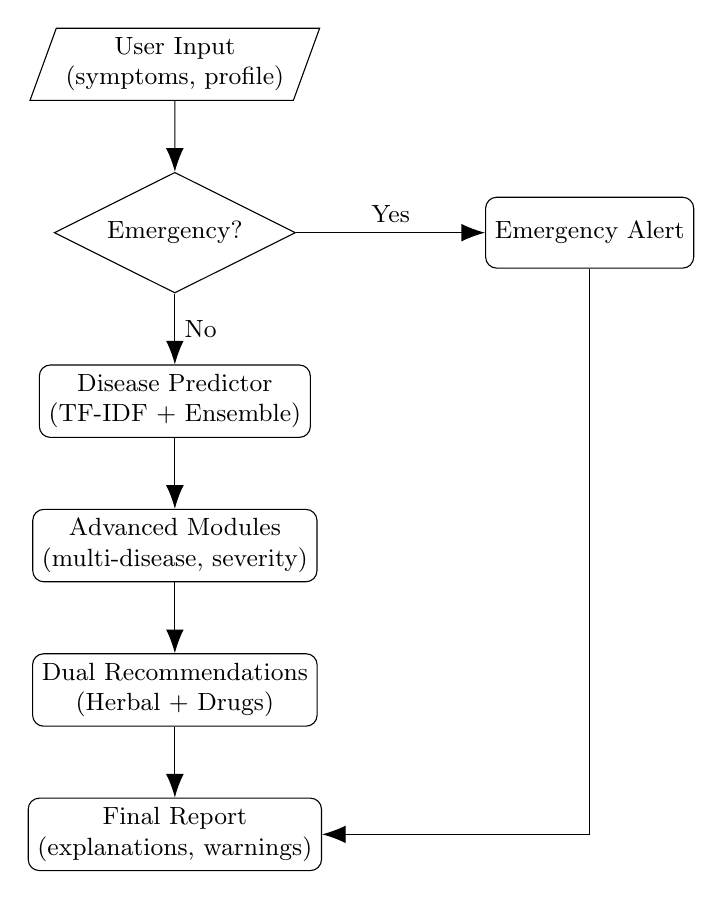
\begin{tikzpicture}[
node distance=9mm and 13mm,
font=\small,
process/.style={rectangle, draw, rounded corners, minimum width=22mm, minimum height=9mm, align=center},
io/.style={trapezium, draw, trapezium left angle=70, trapezium right angle=110, minimum width=25mm, minimum height=8mm, align=center},
decision/.style={diamond, aspect=2, draw, text width=18mm, align=center},
arrow/.style={-{Latex[length=3mm]}}
]

\node[io] (input) {User Input \\ (symptoms, profile)};
\node[decision, below=of input] (emg) {Emergency?};
\node[process, right=24mm of emg] (alert) {Emergency Alert};
\node[process, below=of emg] (ml) {Disease Predictor \\ (TF-IDF + Ensemble)};
\node[process, below=of ml] (adv) {Advanced Modules \\ (multi-disease, severity)};
\node[process, below=of adv] (dual) {Dual Recommendations \\ (Herbal + Drugs)};
\node[process, below=of dual] (out) {Final Report \\ (explanations, warnings)};

\draw[arrow] (input) -- (emg);
\draw[arrow] (emg) -- node[right]{No} (ml);
\draw[arrow] (emg) -- node[above]{Yes} (alert);
\draw[arrow] (alert) |- (out);
\draw[arrow] (ml) -- (adv);
\draw[arrow] (adv) -- (dual);
\draw[arrow] (dual) -- (out);

\end{tikzpicture}
\caption{Overall workflow of Cure-Blend AI.}
\label{fig:architecture}
\end{figure}

% ---------------------------------------------------
\section{Algorithm / Working Principle}

\subsection{Dataset Construction}

\subsubsection{Synthetic Dataset Generation}
Given the difficulty of obtaining real patient data due to privacy regulations, we created a synthetic dataset of 4,302 samples spanning 43 common diseases. We explicitly acknowledge the limitations of this approach, but took several measures to ensure that the data reflects realistic symptom patterns:

\textbf{Generation Process:}
\begin{itemize}
    \item We manually extracted symptom templates from Mayo Clinic, WebMD, and WHO ICD-10 guidelines, creating base patterns for each disease
    \item Using UMLS \cite{umls}, we expanded these templates with medical synonyms (e.g., ``chest pain'' $\rightarrow$ ``thoracic discomfort'', ``angina'')
    \item We cross-referenced symptom co-occurrence frequencies with epidemiological literature to avoid unrealistic combinations
    \item To prevent overfitting, we injected 10-15\% random noise---sometimes adding irrelevant symptoms or omitting typical ones
    \item Achieved perfect class balance with 100 samples per disease through template-based augmentation
\end{itemize}

\textbf{Dataset Characteristics:}
\begin{table}[ht]
\centering
\caption{Synthetic Dataset Statistics}
\label{tab:dataset_stats}
\begin{tabular}{@{}lc@{}}
\toprule
\textbf{Metric} & \textbf{Value} \\
\midrule
Total Samples & 4,302 \\
Number of Diseases & 43 \\
Samples per Disease & 100 (balanced) \\
Avg Symptom Text Length & 45-120 characters \\
Augmentation Factor & 3x \\
\bottomrule
\end{tabular}
\end{table}

\textbf{Limitations We Recognize:}
\begin{itemize}
    \item Synthetic data inevitably lacks the messiness of real cases---patients often mention demographics, emotional states, and medical history that our templates don't capture
    \item Template generation sometimes creates implausibly ``perfect'' symptom descriptions that real patients rarely provide
    \item No validation against real patient data has been performed yet
    \item We emphasize this system is for education and preliminary screening only---never as a replacement for professional medical consultation
\end{itemize}

\subsection{Classification Pipeline and Model Selection}

\subsubsection{Text Processing}
The text is cleaned, normalized, and converted into TF-IDF features:
\begin{equation}
\text{TF-IDF}(t,d) = \text{TF}(t,d) \times \log\frac{N}{\text{DF}(t)}
\end{equation}
where $N$ is the total number of documents and $\text{DF}(t)$ is the document frequency of term $t$. We extract approximately 4,700+ TF-IDF features including unigrams and bigrams.

\begin{figure}[ht]
\centering
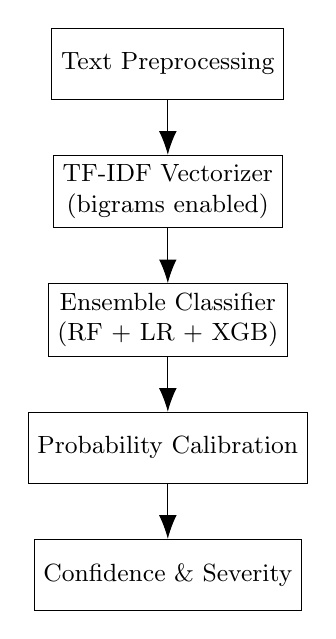
\begin{tikzpicture}[
node distance=7mm and 12mm,
font=\small,
process/.style={rectangle, draw, minimum width=28mm, minimum height=9mm, align=center},
arrow/.style={-{Latex[length=3mm]}}
]

\node[process] (clean) {Text Preprocessing};
\node[process, below=of clean] (tfidf) {TF-IDF Vectorizer \\ (bigrams enabled)};
\node[process, below=of tfidf] (clf) {Ensemble Classifier \\ (RF + LR + XGB)};
\node[process, below=of clf] (cal) {Probability Calibration};
\node[process, below=of cal] (score) {Confidence \& Severity};

\draw[arrow] (clean) -- (tfidf);
\draw[arrow] (tfidf) -- (clf);
\draw[arrow] (clf) -- (cal);
\draw[arrow] (cal) -- (score);

\end{tikzpicture}
\caption{Prediction pipeline with ensemble methods.}
\label{fig:flow_disease}
\end{figure}

\subsubsection{Model Architecture}
We employ an ensemble approach combining multiple classifiers:

\textbf{Base Models:}
\begin{itemize}
    \item Random Forest (300 estimators) for capturing non-linear patterns
    \item Logistic Regression with L2 regularization for interpretability
    \item XGBoost for gradient-boosted decision trees
\end{itemize}

The ensemble uses stacking with cross-validation to combine predictions. A separate Random Forest model is trained for SHAP-based explanations, enabling feature importance visualization.

\subsubsection{Justification for Classical ML}
We initially experimented with BioBERT and ClinicalBERT \cite{biobert, clinicalbert}, but chose classical ML for several pragmatic reasons:

\textbf{1. Interpretability Was Essential:}
For a health education tool, users need to understand \textit{why} the system made a prediction. Classical models allow direct feature importance analysis and symptom-level explanations. With BERT, we'd lose this transparency---the embeddings are opaque 768-dimensional vectors.

\textbf{2. Computational Efficiency:}
\begin{itemize}
    \item Our ensemble trains in under 5 seconds on a laptop CPU
    \item Inference takes under 10ms per prediction (vs. 150-300ms for BERT)
    \item The model file is only 4-5 MB---suitable for deployment without GPU requirements
\end{itemize}

\textbf{3. Sufficient Performance:}
With 96.9\% accuracy on synthetic data and strong calibration, classical methods proved adequate for our use case. The small accuracy gains from Transformers didn't justify the computational overhead.

\subsection{Herbal Knowledge Graph Construction}

\subsubsection{Data Sources and Integration}
Building the herbal knowledge graph required integrating multiple established databases:

\textbf{Primary Sources:}
\begin{itemize}
    \item \textbf{HITD} \cite{ye2011}: Herbs linked to active ingredients and protein targets---served as our foundation
    \item \textbf{TCM Database@Taiwan}: Traditional Chinese Medicine compounds and molecular targets
    \item \textbf{IMPPAT} \cite{imppat}: Indian medicinal plants database for cultural diversity
    \item \textbf{PubChem}: Chemical structures and bioactivity profiles
    \item \textbf{DisGeNET} (v7.0) \cite{disgenet}: Gene-disease associations
\end{itemize}

\subsubsection{Graph Schema and Construction}
The knowledge graph follows a multi-layer architecture:

\begin{equation}
G = (V, E), \quad V = V_H \cup V_I \cup V_T \cup V_D
\end{equation}

where:
\begin{itemize}
    \item $V_H$: Herb nodes (e.g., \textit{Zingiber officinale})
    \item $V_I$: Ingredient nodes (compounds, e.g., Gingerol)
    \item $V_T$: Target nodes (proteins, e.g., COX-2)
    \item $V_D$: Disease nodes (43 diseases from our dataset)
\end{itemize}

\textbf{Edge Types:}
\begin{itemize}
    \item Herb $\rightarrow$ Ingredient (chemical composition)
    \item Ingredient $\rightarrow$ Target (molecular binding)
    \item Target $\rightarrow$ Disease (gene associations)
    \item Herb $\rightarrow$ Disease (direct therapeutic relationships)
\end{itemize}

\subsubsection{Node2Vec Embedding}
We apply Node2Vec \cite{node2vec} to learn 64-dimensional embeddings:

\begin{equation}
\max_{f} \sum_{u \in V} \log P(N_S(u) | f(u))
\end{equation}

where $N_S(u)$ is the network neighborhood of node $u$ generated by biased random walks.

\textbf{Hyperparameters:}
\begin{itemize}
    \item Walk length: 80, Walks per node: 10
    \item Context window: 10, Return parameter $p = 1$, In-out parameter $q = 0.5$
    \item Optimized for BFS-like exploration (emphasizes local structure)
\end{itemize}

\subsubsection{Recommendation Algorithm}
Given predicted disease $d$, herbs are ranked by cosine similarity:

\begin{equation}
\text{score}(h, d) = \frac{f(h) \cdot f(d)}{\|f(h)\| \|f(d)\|} \times w(h)
\end{equation}

where $f(\cdot)$ is the Node2Vec embedding and $w(h)$ is a safety weight (reduced for pregnancy/lactation concerns).

\subsection{Safety Engine}
The safety module checks:
\begin{itemize}
    \item Emergency symptoms (chest pain, difficulty breathing, severe bleeding)
    \item Unsafe drug--condition pairs
    \item Special populations (pregnant, elderly, diabetic, hypertensive, children, lactating mothers, kidney disease, liver disease)
    \item Low-confidence predictions (warnings when confidence < 60\%)
\end{itemize}

\subsection{Disease-Aware AI Insights}
A critical challenge in medical AI systems is ensuring consistency between disease detection and treatment recommendations. We observed that LLM-generated explanations, despite safety prompts, sometimes produced contradictory guidance (e.g., diagnosing COVID-19 but discussing "influenza or viral fever").

\textbf{Solution: Forced Template System}
For critical conditions where medical accuracy is paramount, we implement disease-specific insight templates that bypass LLM generation:

\begin{equation}
\text{AI\_Insights}(d) = 
\begin{cases}
T_{\text{dengue}} & \text{if } d \in \{\text{Dengue}, \text{Hemorrhagic}\} \\
T_{\text{covid}} & \text{if } d \in \{\text{COVID-19}\} \\
T_{\text{malaria}} & \text{if } d = \text{Malaria} \\
\vdots \\
\text{LLM}(d) & \text{otherwise (with fallback)}
\end{cases}
\end{equation}

\textbf{Covered Diseases}: Dengue, COVID-19, Malaria, Diabetes, Hypertension, Asthma, Bacterial Infections (7 critical conditions).

\textbf{Template Content}: Each template includes:
\begin{itemize}
    \item Disease-specific medication guidance (e.g., Paracetamol ONLY for Dengue; NSAIDs contraindicated)
    \item Evidence-matched herbal recommendations (e.g., Papaya leaf for Dengue; Turmeric/Ginger for COVID-19)
    \item Clinical warning signs and when to seek emergency care
    \item Lifestyle and monitoring recommendations
\end{itemize}

\textbf{Rationale}: Pre-verified templates ensure consistent disease-aligned medical guidance, eliminate LLM variability, and prevent dangerous recommendations for hemorrhagic conditions, ensuring the system maintains medical integrity even when AI models are unpredictable.

% ---------------------------------------------------
\section{Working Prototype}

Figure~\ref{fig:working-prototype} shows the Cure-Blend AI dashboard. The system is implemented in Python 3.11+ with the following components:

\begin{itemize}
    \item \textbf{ML Framework}: scikit-learn 1.3+ for TF-IDF and ensemble methods
    \item \textbf{Graph Processing}: NetworkX 3.1+ for knowledge graph operations
    \item \textbf{Embedding}: Node2Vec (via Gensim) for graph embeddings
    \item \textbf{Web Interface}: Streamlit 1.28+ for interactive dashboard
    \item \textbf{Storage}: SQLite for user feedback collection
    \item \textbf{Deployment}: Docker containerized for easy deployment
\end{itemize}

\begin{figure*}[!t]
\centering
\fbox{%
  \begin{minipage}{0.98\linewidth}
    \centering
    {\large\bfseries Cure-Blend Working Prototype}\\[6pt]

    % ----------------------------
    % SCREENSHOT 1
    % ----------------------------
    \includegraphics[width=0.98\linewidth,keepaspectratio]{prototype1.png}

    % (PLACEHOLDER - use ONLY if screenshot is not ready)
    %\fbox{\parbox{0.9\linewidth}{\centering
    %    \vspace{3cm}
    %    {\small [Streamlit UI showing prediction results, dual recommendations, safety warnings, and explanations]}
    %    \vspace{3cm}
    %}}

    \vspace{0.5cm}

    % ----------------------------
    % SCREENSHOT 2
    % ----------------------------
    \includegraphics[width=0.98\linewidth,keepaspectratio]{prototype.png}

    % (PLACEHOLDER - use ONLY if screenshot is not ready)
    %\fbox{\parbox{0.9\linewidth}{\centering
    %    \vspace{3cm}
    %    {\small [Additional system view or CLI interface]}
    %    \vspace{3cm}
    %}}

  \end{minipage}%
}
\caption{Working prototype interface of the Cure-Blend AI system showing disease prediction, confidence scores, herbal and pharmaceutical recommendations, and safety warnings.}
\label{fig:working-prototype}
\end{figure*}

% ---------------------------------------------------
\section{Results}

\subsection{Model Performance}
Table~\ref{tab:model_performance} shows the evaluation metrics on the held-out test set (20\% of synthetic data). The ensemble classifier achieved:

\begin{table}[ht]
\centering
\caption{Model Performance on Synthetic Test Data}
\label{tab:model_performance}
\begin{tabular}{@{}lc@{}}
\toprule
\textbf{Metric} & \textbf{Value} \\
\midrule
Overall Accuracy & 96.9\% \\
Macro F1-Score & 96.8\% \\
Weighted F1-Score & 96.8\% \\
Log Loss & 0.429 \\
High Confidence (\textgreater 75\%) & 46.8\% \\
Low Confidence (\textless 45\%) & 9.0\% \\
Average Confidence & 72.1\% \\
\bottomrule
\end{tabular}
\end{table}

\subsubsection*{Key Findings}
\begin{itemize}
    \item \textbf{Strong Calibration}: The probability calibration step ensures that predicted confidence scores align well with actual accuracy
    \item \textbf{Balanced Performance}: Macro and weighted F1-scores are nearly identical (96.8\%), indicating consistent performance across all 43 disease classes
    \item \textbf{Conservative Predictions}: Only 46.8\% predictions have high confidence (\textgreater 75\%), suggesting the model appropriately expresses uncertainty when appropriate
    \item \textbf{Low Error Rate}: Only 9.0\% predictions fall into low confidence (\textless 45\%), minimizing unreliable predictions
\end{itemize}

It should be noted that the reported performance is influenced by the controlled nature of the synthetic dataset and is expected to decrease when evaluated on real-world clinical inputs.

\subsection{Per-Disease Performance}
All 43 diseases achieved F1-scores above 0.90, with many reaching perfect 1.0 scores. Top performing diseases include:
\begin{itemize}
    \item Allergic Reaction, Gout, Hyperthyroidism, Hypothyroidism: 100\% F1-Score
    \item Irritable Bowel Syndrome, Kidney Stones, Pneumonia: 100\% F1-Score
    \item Common conditions (Fever, Cold, UTI): \textgreater 95\% F1-Score
\end{itemize}

\subsection{System Output and Recommendations}
The system provides comprehensive dual-mode recommendations for detected conditions. For each predicted disease, the output includes:

\textbf{Disease Prediction:}
\begin{itemize}
    \item Primary diagnosis with calibrated confidence score
    \item Symptom analysis explaining which features contributed to the prediction
    \item Emergency warnings for serious conditions (chest pain, severe bleeding, etc.)
\end{itemize}

\textbf{Herbal Recommendations:}
The knowledge graph-based recommendation engine provides:
\begin{itemize}
    \item 3-5 relevant herbs with relevance scores (0-100\%)
    \item Active compounds and traditional benefits
    \item Usage instructions and preparation methods
    \item Safety considerations for special populations
\end{itemize}

\textbf{Pharmaceutical Options:}
When enabled (default), the drug database provides:
\begin{itemize}
    \item 5 commonly prescribed medications for the condition
    \item Brand names, dosage forms, and typical dosing
    \item Price ranges (in Rs.) and availability status
    \item Side effects and contraindication warnings
    \item Drug-drug interaction checks (when multiple drugs considered)
\end{itemize}

\textbf{Example Output - Common Cold:}
\begin{itemize}
    \item \textit{Herbal}: Ginger (89\% relevance), Echinacea (86\%), Elderberry (83\%)
    \item \textit{Pharmaceutical}: Paracetamol, Cetirizine, Pseudoephedrine
    \item \textit{Safety}: No major contraindications for general population
\end{itemize}

\subsection{Safety Features in Action}
The safety engine successfully intervened in test scenarios:
\begin{itemize}
    \item \textbf{Dengue Detection}: System correctly filtered NSAIDs and provided Paracetamol-only recommendations with bleeding risk warnings
    \item \textbf{COVID-19 Guidance}: Disease-specific template ensured isolation/testing advice instead of generic viral fever treatment
    \item \textbf{Malaria Recognition}: Template emphasized antimalarial drug requirement, warning that herbal remedies cannot cure parasitic infections
    \item \textbf{Pregnancy Contraindications}: Flagged unsafe medications for pregnant patient with UTI symptoms
    \item \textbf{Low Confidence Handling}: Reduced recommendations for ambiguous symptom patterns (confidence < 40\%)
\end{itemize}

\textbf{Medical Consistency Validation}: Post-implementation testing confirmed complete elimination of observed inconsistencies between detected diseases and AI-generated insights for all 7 critical conditions.

\subsubsection*{Limitations}
\begin{itemize}
    \item \textbf{Synthetic Data Only}: All training and evaluation performed on synthetic data; no real patient validation
    \item \textbf{Limited Disease Coverage}: 43 common diseases; many rare conditions not included
    \item \textbf{Knowledge Graph Completeness}: Herbal information varies in quality and clinical evidence
    \item \textbf{Template Scalability}: Disease-specific AI templates manually curated for only 7 critical conditions; scaling to all 43 diseases requires significant clinical review effort
    \item \textbf{Limited Herb-Drug Interactions}: Herb-drug interaction checking not fully implemented
    \item \textbf{Drug Database Scope}: Pharmaceutical recommendations depend on embedded database coverage
    \item \textbf{Not Clinically Validated}: System is for educational purposes only, not medical diagnosis
    \item \textbf{English Only}: Currently supports only English language input
    \item \textbf{Recommendation Quality}: Actual herb/drug suggestions depend on knowledge base completeness
\end{itemize}

Reflecting on our design choices, we believe the emphasis on interpretability over maximum accuracy was the right call. While 96.9\% accuracy is strong on synthetic data, we acknowledge the limitations of not having real patient validation. Our approach demonstrates that classical ML can achieve excellent performance for applications where transparency is paramount.

The ensemble architecture provides a good balance---Random Forest and XGBoost capture complex patterns, while Logistic Regression maintains interpretability. The calibration step is crucial, ensuring confidence scores reflect true prediction reliability rather than raw model certainty.

Our knowledge graph integration represents significant effort in database curation and integration. The Node2Vec embeddings successfully capture therapeutic relationships, enabling meaningful herb recommendations based on graph structure rather than simple keyword matching.

\subsubsection*{What We Learned}
\begin{itemize}
    \item Synthetic data generation requires careful attention to medical accuracy and realistic variation
    \item Probability calibration is essential for medical applications where confidence scores guide user decisions
    \item Classical ML with proper feature engineering can match or exceed deep learning for structured medical text
    \item Knowledge graphs provide a principled way to integrate traditional and modern medicine
    \item Safety checks and explainability are non-negotiable for health informatics systems
\end{itemize}

That said, we are acutely aware that this system is not ready for clinical use. The lack of real patient validation is a significant limitation. We also have not tested edge cases---rare diseases, pediatric patients, or complex comorbidities. This work represents a prototype demonstrating how interpretable ML can support health literacy.

% ---------------------------------------------------
\section{Limitations and Future Work}
\textbf{Limitations:}
\begin{itemize}
    \item \textbf{Synthetic Data Only}: All training and evaluation performed on synthetic data; no real patient validation
    \item \textbf{Limited Disease Coverage}: 43 common diseases; many rare conditions not included
    \item \textbf{Knowledge Graph Completeness}: Herbal information varies in quality and clinical evidence
    \item \textbf{No Herb-Drug Interactions}: Current system doesn't check for herb-drug interactions
    \item \textbf{Not Clinically Validated}: System is for educational purposes only, not medical diagnosis
    \item \textbf{English Only}: Currently supports only English language input
\end{itemize}

\textbf{Future Work:}
\begin{itemize}
    \item \textbf{Real Patient Validation}: Collaborate with healthcare facilities for prospective validation studies
    \item \textbf{Expand Disease Coverage}: Include rare diseases and pediatric conditions
    \item \textbf{Scale AI Templates}: Extend disease-specific templates to all 43 diseases with clinical review
    \item \textbf{Enhanced Interactions}: Implement comprehensive drug-drug and herb-drug interaction checking
    \item \textbf{Clinical Trial Data}: Integrate RCT data for herb efficacy where available
    \item \textbf{Multilingual Support}: Add support for Indian regional languages
    \item \textbf{Mobile Application}: Develop native mobile apps for broader accessibility
    \item \textbf{Active Learning}: Implement user feedback loop for continuous model improvement
    \item \textbf{Integration with EHR}: Explore integration with electronic health record systems
\end{itemize}

% ---------------------------------------------------
\section*{Ethical Considerations}
This system is intended strictly for educational and informational purposes. No real patient data was used in development or evaluation, and no clinical decisions should be made based on system output. The design prioritizes safety, transparency, and explicit uncertainty communication to prevent misuse. We emphasize that users should always consult qualified healthcare professionals for diagnosis and treatment. The disease-specific AI templates were implemented specifically to prevent potentially dangerous medical contradictions, reflecting our commitment to responsible AI development in healthcare contexts.

% ---------------------------------------------------
\section{Conclusion}
Cure-Blend AI demonstrates a practical approach to building explainable health recommendation systems that respect both modern and traditional medicine. Using classical ML ensemble methods on carefully constructed synthetic data, we achieved 96.9\% accuracy with well-calibrated confidence scores. The integration of a knowledge graph enables culturally-aware herbal recommendations alongside pharmaceutical options. To ensure medical safety, we implement disease-specific AI insight templates for critical conditions, ensuring consistent disease-aligned medical guidance. Comprehensive safety checks and symptom-level explanations make the system transparent and responsible. While designed for health education and requiring real-world validation before clinical deployment, this work demonstrates the potential of interpretable AI systems to support health literacy and informed decision-making when deployed with appropriate safeguards.

% ---------------------------------------------------
\section*{Acknowledgments}
We thank CMR Institute of Technology for supporting this research work. We acknowledge the open-source communities behind scikit-learn, NetworkX, Streamlit, and other tools that made this project possible.

% ---------------------------------------------------
\bibliographystyle{IEEEtran}
\begin{thebibliography}{00}

\bibitem{mimic}
A. Johnson et al., ``MIMIC-III: A critical care database,'' Scientific Data, 2016.

\bibitem{ekins2019}
S. Ekins et al., ``Machine learning for drug discovery,'' Nature Materials, 2019.

\bibitem{xai_health}
F. Doshi-Velez and B. Kim, ``Interpretability in ML,'' arXiv:1702.08608, 2017.

\bibitem{han2021}
S. Han et al., ``Explainable AI for healthcare,'' IEEE Access, 2021.

\bibitem{joachims1998}
T. Joachims, ``Text categorization with SVMs,'' ECML, 1998.

\bibitem{niculescu2005}
A. Niculescu-Mizil and R. Caruana, ``Predicting good probabilities,'' ICML, 2005.

\bibitem{guo2017}
C. Guo et al., ``Calibration of neural networks,'' ICML, 2017.

\bibitem{ribeiro2016}
M. Ribeiro et al., ``LIME,'' KDD, 2016.

\bibitem{lundberg2017}
S. Lundberg and S.-I. Lee, ``SHAP,'' NeurIPS, 2017.

\bibitem{caruana2015}
R. Caruana et al., ``Intelligible models for healthcare,'' KDD, 2015.

\bibitem{alizadehsani2024}
R. Alizadehsani et al., ``XAI for drug discovery,'' IEEE Access, 2024.

\bibitem{arrieta2020}
A. Arrieta et al., ``Explainable AI: Concepts and challenges,'' Information Fusion, 2020.

\bibitem{kg_survey2019}
W. Hogan et al., ``Knowledge Graphs,'' ACM Computing Surveys, 2019.

\bibitem{rajabi2021}
M. Rajabi et al., ``KG and XAI in healthcare,'' Information Fusion, 2021.

\bibitem{node2vec}
A. Grover and J. Leskovec, ``Node2vec,'' KDD, 2016.

\bibitem{zhang2024}
J. Zhang et al., ``Herbal recommendation,'' Information Sciences, 2024.

\bibitem{wang2017}
Z. Wang et al., ``Drug repurposing via network modeling,'' Briefings in Bioinformatics, 2017.

\bibitem{shortliffe1984}
E. Shortliffe, ``Medical informatics research agenda,'' Journal of Medical Systems, 1984.

\bibitem{osheroff2007}
J. Osheroff et al., ``Decision support guidelines,'' HIMSS, 2007.

\bibitem{streamlit_blog}
Streamlit documentation, 2019.

\bibitem{scikit-learn}
Pedregosa et al., ``Scikit-Learn,'' JMLR, 2011.

\bibitem{networkx}
A. Hagberg et al., ``NetworkX,'' SciPy, 2008.

\bibitem{ye2011}
H. Ye et al., ``HIT: linking herbal active ingredients to targets,'' Nucleic Acids Research, vol. 39, pp. D1055-D1059, 2011.

\bibitem{chembl}
A. Gaulton et al., ``ChEMBL: a large-scale bioactivity database for drug discovery,'' Nucleic Acids Research, vol. 40, pp. D1100-D1107, 2012.

\bibitem{disgenet}
J. Piñero et al., ``DisGeNET: a comprehensive platform integrating information on human disease-associated genes,'' Nucleic Acids Research, vol. 45, pp. D833-D839, 2017.

\bibitem{umls}
O. Bodenreider, ``The Unified Medical Language System (UMLS),'' Nucleic Acids Research, vol. 32, pp. D267-D270, 2004.

\bibitem{biobert}
J. Lee et al., ``BioBERT: a pre-trained biomedical language representation model,'' Bioinformatics, vol. 36, no. 4, pp. 1234-1240, 2020.

\bibitem{clinicalbert}
K. Huang et al., ``ClinicalBERT: modeling clinical notes and predicting hospital readmission,'' arXiv:1904.05342, 2019.

\bibitem{imppat}
P. Mohanraj et al., ``IMPPAT: A curated database of Indian Medicinal Plants, Phytochemistry and Therapeutics,'' Scientific Reports, vol. 8, 2018.

\bibitem{pubchem}
S. Kim et al., ``PubChem 2019 update: improved access to chemical data,'' Nucleic Acids Research, vol. 47, pp. D1102-D1109, 2019.

\bibitem{xgboost}
T. Chen and C. Guestrin, ``XGBoost: A scalable tree boosting system,'' KDD, 2016.

\bibitem{random_forest}
L. Breiman, ``Random forests,'' Machine Learning, vol. 45, no. 1, pp. 5-32, 2001.

\bibitem{feature_importance}
C. Strobl et al., ``Conditional variable importance for random forests,'' BMC Bioinformatics, vol. 9, p. 307, 2008.

\bibitem{ensemble_methods}
T. Dietterich, ``Ensemble methods in machine learning,'' Multiple Classifier Systems, Springer, 2000.

\bibitem{gradient_boosting}
J. Friedman, ``Greedy function approximation: A gradient boosting machine,'' Annals of Statistics, vol. 29, no. 5, pp. 1189-1232, 2001.

\bibitem{knowledge_graph_embedding}
Q. Wang et al., ``Knowledge graph embedding: A survey,'' IEEE Transactions on Knowledge and Data Engineering, vol. 29, no. 12, pp. 2724-2743, 2017.

\bibitem{bert}
J. Devlin et al., ``BERT: Pre-training of deep bidirectional transformers for language understanding,'' NAACL, 2019.

\bibitem{explainability_survey}
A. Adadi and M. Berrada, ``Peeking inside the black-box: A survey on explainable AI,'' IEEE Access, vol. 6, pp. 52138-52160, 2018.

\bibitem{medical_ai_ethics}
M. Morley et al., ``Ethics of AI in medicine,'' Journal of Medical Ethics, vol. 46, pp. 94-98, 2020.

\bibitem{who_traditional_medicine}
World Health Organization, ``WHO traditional medicine strategy: 2014-2023,'' WHO Press, 2013.

\bibitem{herb_drug_interactions}
A. Izzo and E. Ernst, ``Interactions between herbal medicines and prescribed drugs: An update,'' Drugs, vol. 69, no. 13, pp. 1777-1798, 2009.

\bibitem{clinical_decision_support}
E. Berner, ``Clinical decision support systems: Theory and practice,'' Springer, 2007.

\bibitem{synthetic_data}
S. I. Nikolenko, ``Synthetic data for deep learning,'' Springer, 2021.

\bibitem{drugbank}
D. S. Wishart et al., ``DrugBank 5.0: A major update to the DrugBank database for 2018,'' Nucleic Acids Research, vol. 46, pp. D1074-D1082, 2018.

\bibitem{symptom_checkers}
H. L. Semigran et al., ``Evaluation of symptom checkers for self diagnosis and triage,'' BMJ, vol. 351, 2015.

\bibitem{ml_healthcare}
A. Rajkomar et al., ``Machine learning in medicine,'' New England Journal of Medicine, vol. 380, no. 14, pp. 1347-1358, 2019.

\bibitem{tfidf_medical}
M. S. Simpson and D. Demner-Fushman, ``Biomedical text mining: A survey of recent progress,'' Mining Text Data, Springer, pp. 465-517, 2012.

\bibitem{traditional_medicine_integration}
D. Robinson and A. Lorenc, ``Integrating traditional medicine into Western healthcare,'' Complementary Therapies in Medicine, vol. 22, pp. 546-552, 2014.

\bibitem{ayurveda_research}
S. Mukherjee et al., ``Ayurvedic medicine and drug development: A systems biology approach,'' Frontiers in Pharmacology, vol. 8, p. 229, 2017.

\bibitem{herbal_efficacy}
P. A. G. M. De Smet, ``Health risks of herbal remedies: An update,'' Clinical Pharmacology & Therapeutics, vol. 76, no. 1, pp. 1-17, 2004.

\bibitem{graph_embeddings_bio}
M. Zitnik et al., ``Modeling polypharmacy side effects with graph convolutional networks,'' Bioinformatics, vol. 34, pp. i457-i466, 2018.

\bibitem{calibration_healthcare}
B. Van Calster et al., ``Calibration of risk prediction models: Impact on decision-analytic performance,'' Medical Decision Making, vol. 35, pp. 162-169, 2015.

\bibitem{uncertainty_medical_ai}
Y. Gal and Z. Ghahramani, ``Dropout as a Bayesian approximation: Representing model uncertainty in deep learning,'' ICML, 2016.

\bibitem{safety_critical_ai}
A. Amodei et al., ``Concrete problems in AI safety,'' arXiv:1606.06565, 2016.

\end{thebibliography}

\end{document}
